\chapter{Discovery Potential \Contact{Francis-Yan}}
\label{sec:discovery}
\bigskip
\Contributors{Keith Bechtol, Francis-Yan Cyr-Racine, William A.\ Dawson, Alex Drlica-Wagner, Cora Dvorkin, Vera Gluscevic, Manoj Kaplinghat, Casey Lam, Jessica Lu, Michael Medford, Ethan O.\ Nadler, J.\ Anthony Tyson}

Cosmology has a long history of testing particle models of dark matter.
For instance, neutrinos were long considered a viable dark matter candidate \citep[\eg,][]{Kolb:1988}, before precise cosmological measurements made it clear that the universe contains multiple invisible components.
The 30\eV neutrino dark matter candidate is an especially interesting case study of the interplay between particle physics experiments and astrophysical observations.
\citet{Lyubimov:1980un} reported the discovery of a non-zero neutrino rest mass in the range $14\eV < m_{\nu} < 46\eV$ which was subsequently tested by several other tritium $\beta$-decay experiments over the next decade.
Neutrinos with this mass would provide a significant fraction of the critical energy density needed to close the universe, but would be relativistic at the time of decoupling (\ie, hot dark matter).
During the same period, the first stellar velocity dispersion results for dwarf spheroidal galaxies showed that these galaxies are highly dark matter dominated.
The inferred dark matter density within the central regions of the dwarfs was used to place lower limits on the neutrino rest mass that were incompatible with the 30\eV neutrino dark matter candidate \citep{Aaronson:1983,Gerhard:1992}.
Similar stories can be told of heavy leptons \citep[\eg,][]{Gunn:1978}, \CHECK{and other dark matter candidates}, which have been excluded by cosmological and astrophysical measurements.
Cosmology has continually shown that it is impossible to separate the \emph{macroscopic distribution} of dark matter from the \emph{microscopic physics} governing dark matter.

Through much of this work, we have expressed sensitivity to dark matter microphysics in terms of upper limits in the case of non-detection of deviations from the baseline CDM paradigm.
In this section, we consider two potential astrophysical discovery scenarios for non-minimal dark matter properties that could be realized in the LSST era.
In each scenario, a critical question is whether the systematic uncertainties associated with conventional astrophysical processes can be controlled at a level that would be sufficiently compelling to guide non-gravitational dark matter searches with collider, direct, and indirect detection experiments.

\section{Compact Object Discovery}
\label{sec:pbh_discovery}
\Contributors{William A.\ Dawson, Jessica Lu, Casey Lam, Michael Medford, Alex Drlica-Wagner}

While current constraints make it unlikely that all of dark matter is composed of compact objects with a monochromatic mass function and a uniform spatial distribution, it is nearly certain that LSST will measure the mass spectrum of Galactic black holes (\figref{macho_discovery}).
In this regime, it will be necessary to test whether the observed black hole population statistics can be explained through stellar evolution, or if a novel black hole production mechanism is required (\ie, PBHs).
The discovery of an excess component to the black hole population will necessarily require a fit of the underlying population of stellar remnants and the associated astrophysical systematics. 
However, an excess of high-mass black holes ($M \gtrsim 30\Msun$) or the discovery of black hole clusters \citep[\eg,][]{Clesse:2016} could provide a smoking gun for PBH detection.
If such a PBH population is discovered, it will be possible to measure not only the fraction of dark matter in compact objects, but the compact object mass spectrum, which will in turn set constraints on the spectrum of perturbations during and after inflation \citep[\eg,][]{1702.03901}.
Knowing that some fraction of the dark matter exists as PBHs will force a re-interpretation of particle physics limits from direct and indirect searches.
Preferred regions of WIMP parameter space that are excluded under the assumption that WIMPs comprise all the dark matter will be reopened.
Somewhat counter-intuitively, the outlook for the WIMP may be stronger in a universe where PBHs make up some fraction of the dark matter density.

In \figref{macho_discovery}, we follow the analysis of \citet{Lu:2019} to present an illustration of the LSST discovery potential for a population of high-mass black holes.
\citet{Lu:2019} calculated the expected microlensing event rate from stars and stellar-mass compact objects in a $3.74 \deg^2$ field in the direction of the Galactic bulge.
In addition, a population of high-mass black holes was injected with a Gaussian mass distribution centered at $30\Msun$ with a standard deviation of $20\Msun$.
For simplicity, the injected population was assumed to have the same spatial and velocity distribution as Milky Way halo stars.
The mass density (and hence number density) of injected black holes was scaled to match 5\%, 15\%, and 30\% of the Milky Way dark matter halo.
We scale the microlensing rates from \citet{Lu:2019} to a $10\deg \times 10\deg$ Galactic bulge field, which could be observed as part of a devoted LSST mini-survey.
The resulting total microlensing event rates are shown in \figref{macho_discovery}.
The number of detectable microlensing events will subject to the LSST microlensing detection efficiency, which is expected to be $\gtrsim 1\%$ for events with $t_{\rm E} > 100$\,days \citep{Lu:2019}.
This analysis does not include the added sensitivity long-duration microlensing events from the parallax effects described in \secref{microlensing}. 
Astrometric microlensing described in \secref{astrometric_microlens} will be important for breaking the mass-distance degeneracy of the lens.

\begin{figure}[t]
\centering
%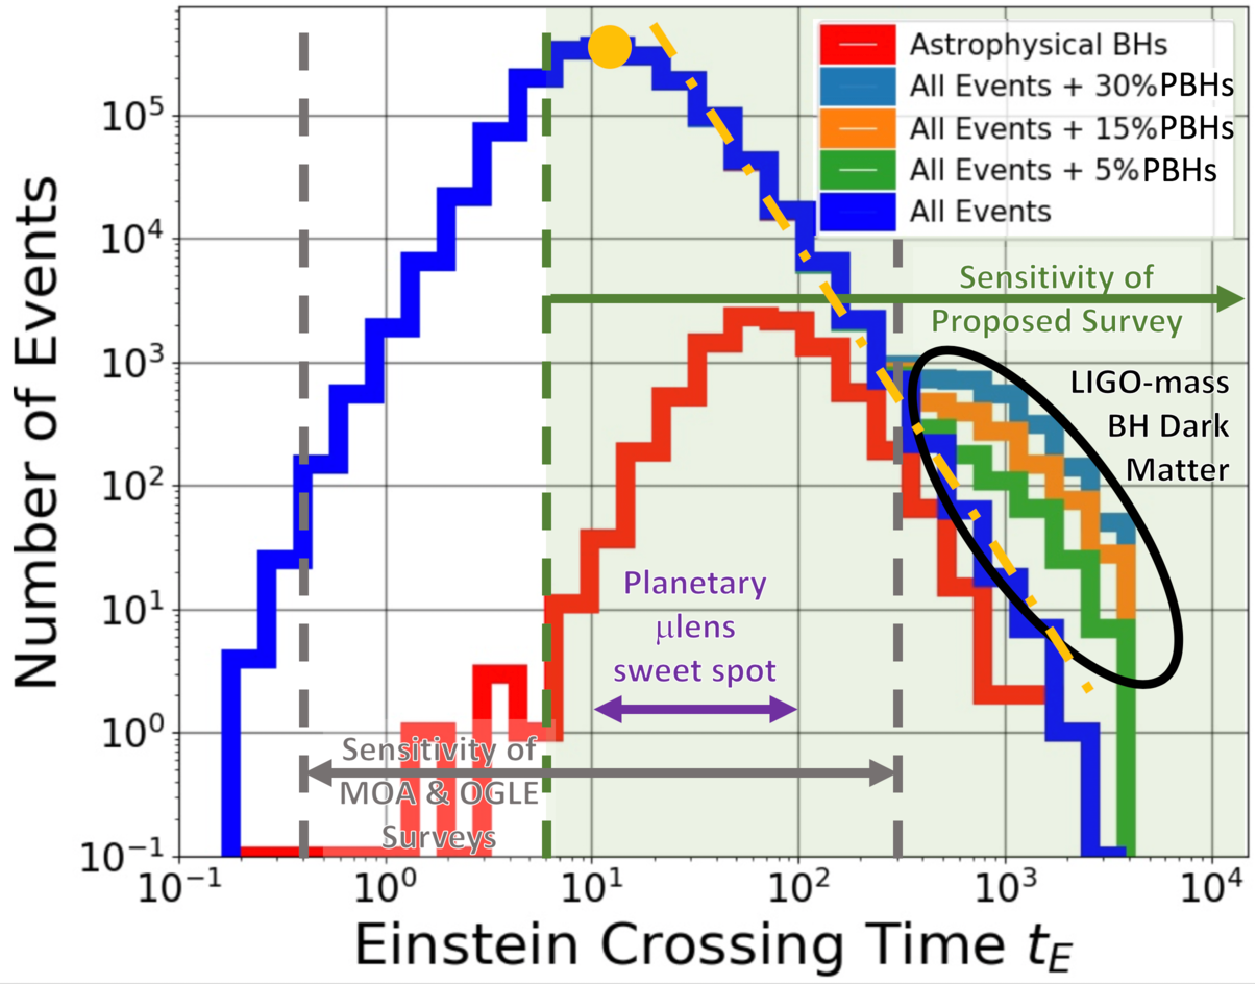
\includegraphics[width=0.6\columnwidth]{nevents_vs_t.pdf}
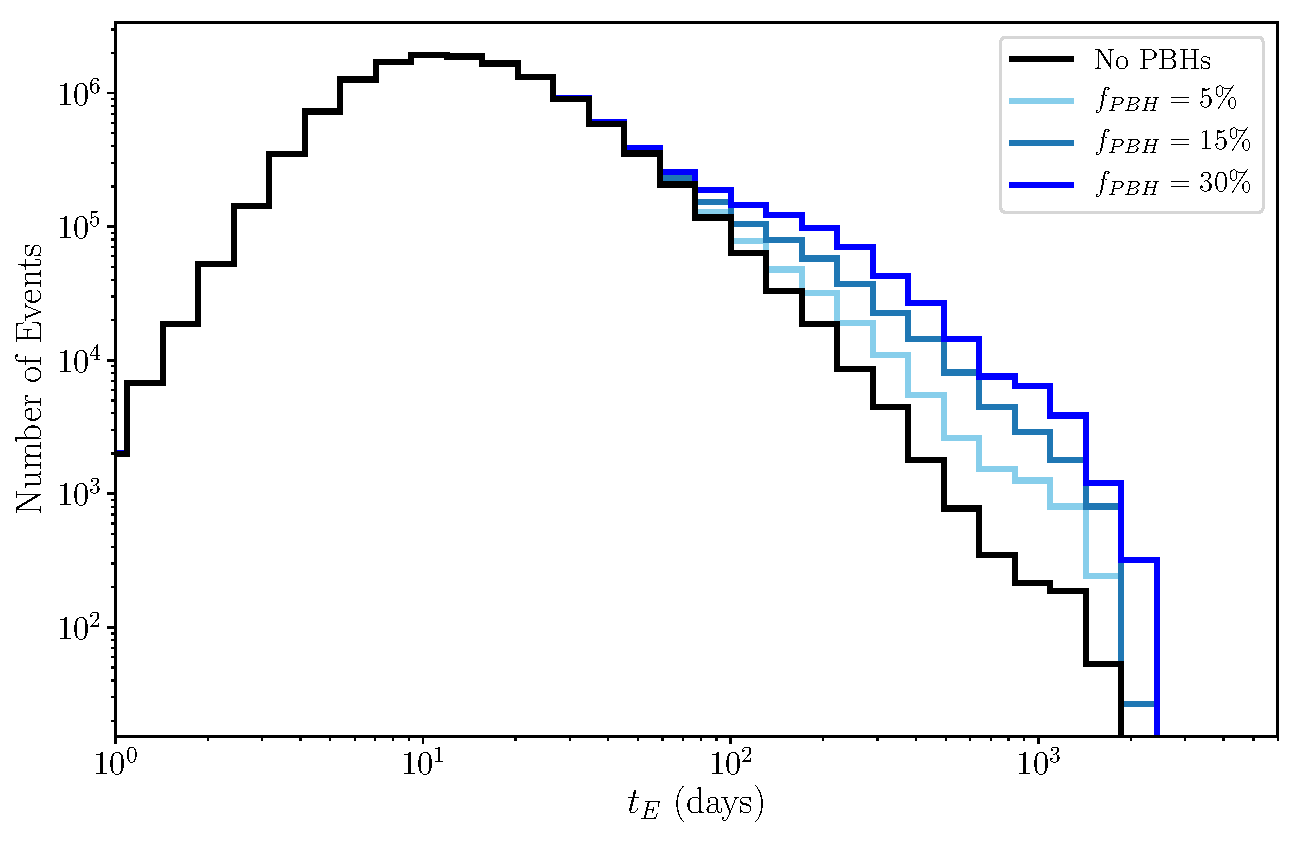
\includegraphics[width=0.75\columnwidth]{macho_discovery.pdf}
\caption{\label{fig:macho_discovery}
  The expected number of $<\,2\theta_\mathrm{E}$ microlensing events scaled to a $10 \deg \times 10 \deg$ bulge field.
  The microlensing rate from astrophysical source (stars and compact objects resulting from stellar evolution) is shown in black.
  Blue histograms show the expected microlensing rate assuming different fractions of dark matter composed of LIGO-mass black holes (see text for details).
 The LSST detection efficiency is expected to be $\gtrsim 1\%$ for $t_{\rm E} > 100$\,days \citep[see][for details]{Lu:2019}.
}
\end{figure}

\section{WDM/SIDM Discovery}
\label{sec:wdm_sidm_discovery}
\Contributors{Francis-Yan Cyr-Racine, Ethan O.\ Nadler, Keith Bechtol, Vera Gluscevic, Alex Drlica-Wagner, Manoj Kaplinghat}

We now turn to the scenario in which dark matter possesses a particle mass or self-interaction cross section that would partially account for observed small-scale structure anomalies.
There are currently several hints of non-minimal dark matter particle properties arising from comparisons between theoretical predictions and observed galaxy populations at the dwarf galaxy scale, \ie, distances below $1 \Mpc$ and mass scales below $10^{11} \Msun$ \citep[reviewed by][]{BuckleyPeter:2017,Bullock:2017}.
However, the interpretation of these discrepancies in terms of dark matter microphysics has been hindered by uncertainties in the mapping between visible stellar populations and dark matter halos, which involves both the physics of galaxy formation as well as the connection between observable and intrinsic galaxy properties (see \secref{smallest_galaxies} and \secref{halo_profile_group}).
In a regime where systematic uncertainties are already important, it is reasonable to ask how the increased statistical power of LSST will help to resolve our current small-scale structure quandary.

We argue here that the decisive advantage of LSST is the opportunity to combine an ensemble of astrophysical dark matter probes that offer complementary perspectives on dark matter halo abundances and profile shapes, and which are affected by different sources of systematic uncertainty.
For the purpose of illustration, we outline a possible ``roadmap to discovery'' for a dark matter model that produces a cutoff in the matter power spectrum and a suppression of the central dark matter profile just below the current sensitivity limit---\ie, $\Mhm \simeq 10^{8}\Msun$.
As a concrete example, we assume that these astrophysical features result from a dark matter particle model with a self-interaction cross section of $\sigmam = 2 \cmg$ and a thermal particle mass of $\mWDM = 6 \keV$.

The first indication of a discrepancy with CDM might come shortly after the first public data release of LSST survey data when automated searches for Milky Way satellites reveal only a handful of new candidate ultra-faint galaxies. 
Using the framework described in \secref{smallest_galaxies}, these observations could be combined to derive bounds on the WDM mass and the minimum halo mass for galaxy formation, $\mathcal{M}_{\rm min}$. These constraints would deviate significantly from expectations derived from CDM and the observational sensitivity of LSST, thereby hinting at a preference for new physics.

The combined depth and sky coverage of LSST will also enable the study of dwarf galaxy satellite populations around other hosts out to several Mpc, as well as the ``field'' population of isolated dwarf galaxies.
By detecting a statistical sample of low-luminosity galaxies in a wide variety of environments, LSST will provide a wealth of input data to theoreticians developing galaxy formation simulations.
In our hypothetical scenario, numerical simulations will show that it is challenging to solve the dearth of observed satellite galaxies by tuning baryonic physics models (\eg, reionization physics, supernova feedback, galaxy formation threshold).

The same LSST data set is expected to reveal many new stellar streams and gravitational lens systems, which would provide access to dark matter halos below the mass threshold of galaxy formation (\secref{stream_gaps} and \secref{stronglens}).
The search for stream gaps and lensing anomalies would be particularly well motivated since these systems would probe a halo mass regime where the discrepancy with CDM would be even more severe.
In addition, these halos are largely devoid of baryons and would be subject to different astrophysical and observational systematics.
We could expect a period of several years necessary to collect and analyze follow-up observations (both spectroscopy and high-resolution imaging) of the most favorable stream and lens systems.
The absence of lower-mass dark matter halos would greatly increase the tension between observations and the predictions of CDM.
In addition, it will be difficult to explain a dearth of dwarf galaxies and lower-mass halos with the same astrophysical systematics, strengthening the case for a fundamental physics explanation.


In parallel, spectroscopic follow-up of LSST-discovered Milky Way satellites with other telescopes (\secref{MW_sats_spec}) will probe their inner density profiles and provide further information about a possible matter power spectrum cutoff or dark matter self-interaction. These dynamical measurements might reveal an unexpected diversity in central densities measurements that might be difficult to explain within the CDM framework. In particular, the discovery of exceptionally dense or exceptionally diffuse ultra-faint satellites with properties that correlate with their orbital parameters could provide a measurement of the SIDM cross section at low velocities \citep{Nishikawa:2019lsc}. Furthermore, density profile measurements of larger dwarf galaxies outside the Milky Way using weak lensing data from LSST (\secref{halo_profile_group}) could probe the SIDM cross section in a different velocity regime. Similarly, the (non-)observation of deviations in halo profiles of galaxy clusters will be able to inform the velocity dependence of the SIDM cross section.


While much work is still needed to combine all these different probes of dark matter properties (see next section), it is informative to consider what a discovery of our fiducial non-CDM model ($\sigmam = 2 \cmg$, $\mWDM = 6 \keV$) might look like quantitatively with LSST-discovered Milky Way satellite systems. To do so, we use the galaxy-halo connection model outlined in \citet{Nadler:2018} to generate mock LSST observations of faint satellites, and use a similar procedure to that described in \secref{combine_probes} to capture the impact of self-interaction and a mass function cut-off on the central densities of these objects. We construct a binned likelihood in the space of stellar dispersion and luminosity and jointly fit for $\sigmam$ and $\mWDM$, marginalizing over several galaxy-halo connection and Milky Way host halo nuisance parameters. Using a LSST detection threshold for Milky Way satellites of $M_V = 0$ mag and $\mu=32$ mag/arcsec$^2$, we obtain the simultaneous measurement of the SIDM cross section and WDM particle mass presented in \figref{sidm_wdm_disc}. Here, the sensitivity to $\mWDM$ stems primarily from the lower number of faint satellites that the mock LSST observations contain compared the the CDM prediction, while the SIDM cross section sensitivity is driven by the diversity of central densities in the mock observations for $\sigmam = 2 \cmg$. Degeneracy with the halo mass threshold for galaxy formation causes the long tail towards large dark matter mass. Importantly, such degeneracy could be broken by combining these satellite measurements with a probe that is independent of subhalo luminosity such as stellar stream gaps or strong lensing, ultimately resulting in closed contours at high statistical significance. This would signify the start of an era of precision measurement of dark matter particle properties using astrophysical observations.

\begin{figure}
\centering
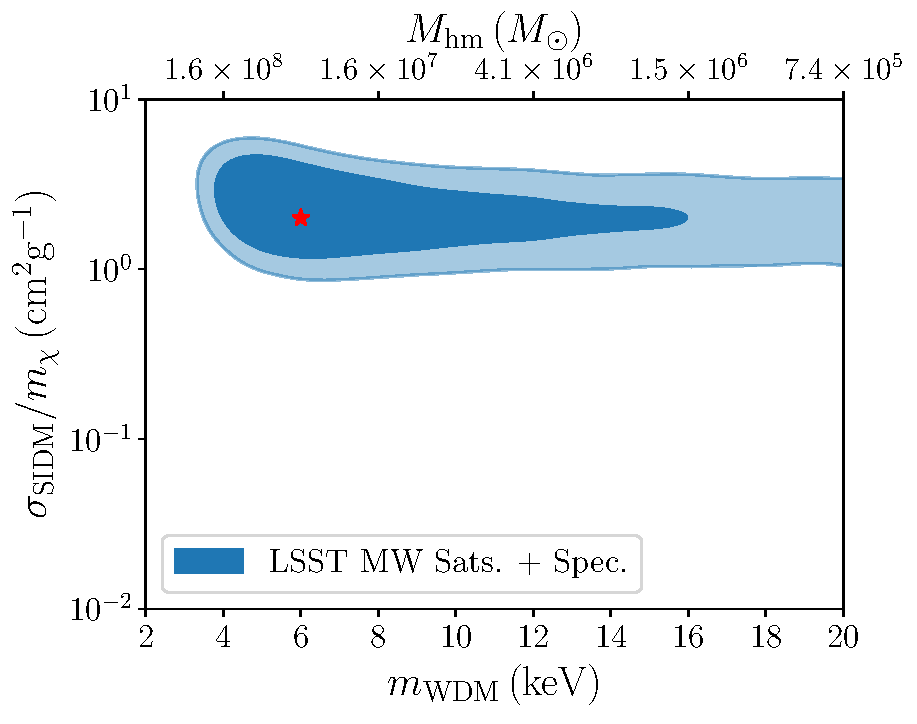
\includegraphics[width=0.75\columnwidth]{figures/WDM_SIDM_discovery_test.pdf}
\caption{\label{fig:sidm_wdm_disc} Example of a measurement of particle properties for a dark matter model with a self-interaction cross section and matter power spectrum cut-off just beyond current constraints ($\sigmam = 2 \cmg$ and $\mWDM = 6\keV$, indicated by the red star). Contours are created by following a procedure similar to \citet{Nadler:2018}, but augmented with the model outlined in \secref{combine_probes} to capture the effect of a power spectrum cut-off and a nonzero self-interaction cross section on the central densities of LSST-discovered Milky Way satellites with spectroscopic follow-up. We take $M_V=0$ mag and $\mu=32$ mag/arcsec$^2$ as our detection threshold for LSST. We assume a prior on the WDM mass $\propto 1/\mWDM$, and a prior on the Milky Way mass from \citet{Callingham:2018vcf}. This figure should be interpreted as a suggestive illustration of the dark matter science that will be enabled by LSST, rather than a precise forecast.  
}
\end{figure}

\vspace{1em} \noindent {\bf Roadmap to measurement}

The hypothetical discovery scenario described above would transform the field of astrophysical dark matter research from one of constraint to one of measurement.
In the measurement paradigm, complementary dark matter probes would be combined to break degeneracies in dark matter models and to constrain astrophysical systematics.
Such analyses would necessitate a probabilistic inference framework to self-consistently analyze multiple measurements probing the same underlying dark-matter physics. 
Such a likelihood-based framework is commonplace for modern cosmological parameter estimation with data from the CMB and current galaxy surveys, and is already under development for dark energy studies with LSST \citep{DESC:CCL}\footnote{\url{https://github.com/LSSTDESC/CCL}}. 
The extension of such a framework to the strongly non-linear regime of dark matter physics in small-scale structures will necessarily rely upon the development of physically accurate and numerically efficient procedures to simulate or emulate the observable effects resulting from varying fundamental properties of dark matter.
Such investigations have already begun through rigorous cosmological simulation of structure formation in WDM, SIDM, and FDM scenarios \citep[\eg,][]{Lovell:2013ola,Dooley:2016ajo,1807.06018,1811.11791}; however, to incorporate these results in a likelihood fit, it will be necessary to evolve effective theories of structure formation \citep[\eg,][]{Cyr-Racine:2015ihg} or quick emulation techniques.
From the data analysis side, recent studies of Milky Way satellite galaxies \citep[\eg,][]{Jethwa:2018,Nadler:2018} have begun to pave the way toward probabilistic analyses of small-scale structure, with the aim of robustly probing both galaxy physics and fundamental physics.
As these and other analyses continue to advance, it will become possible to combine likelihood functions and parameter chains from multiple different observables into a self-consistent likelihood framework. 
This likelihood space can then be scanned to produce joint constraints on dark matter properties.

The self-consistent inclusion of all available information in a joint-likelihood framework will boost the statistical significance of a combined measurement, robustly include astrophysical systematics, and break degeneracies between astrophysics and dark matter models.
The development of fast techniques to predict changes in astrophysical observables from changes to fundamental dark matter properties will allow the production of an end-to-end forward modeling framework for statistical inference.
The ability to simultaneously fit \textit{all} astrophysical observables with \emph{the same} non-minimal dark matter model, while rigorously marginalizing over relevant astrophysical systematics, will produce a compelling argument for the discovery of new dark matter physics.
The same statistical parameter estimation framework will quantify model degeneracies and enable rigorous statements about dark matter particle properties.
These results will critically guide the experimental particle physics program in a post-discovery era.


\section{Outlook}
\label{sec:outlook}
\Contributors{Alex Drlica-Wagner, Keith Bechtol, Vera Gluscevic, J. Anthony Tyson}

More than 80 years after its astrophysical discovery, the fundamental nature of dark matter remains one of the foremost open questions in physics.
Over the last several decades, an extensive experimental program has sought to determine the cosmological origin, fundamental constituents, and interaction mechanisms of dark matter. 
While the existing experimental program has largely focused on weakly-interacting massive particles, there is strong theoretical motivation to explore a broader set of dark matter candidates.
LSST provides a unique, powerful, and complementary platform to study the fundamental physics of dark matter.

LSST will detect and study the smallest dark matter halos, thereby probing the minimum mass of ultra-light dark matter and thermal warm dark matter.
Precise measurements of the density and shapes of dark matter halos will probe dark matter self-interactions, thereby accessing hidden sector and dark photon models.
Microlensing measurement have the potential to detect primordial black holes and to probe the physics of inflation at ultra-high energy scales.
Anomalous energy loss from axion-like particles could reveal itself through precise measurements of stellar populations.
In addition, LSST can uniquely test for correlations between dark matter and dark energy.

Finally, and perhaps most critically, the multi-faceted LSST data will allow novel probes of dark matter physics that have yet to be considered.
These new ideas are especially important as the absence of evidence for the most popular dark matter candidates continues to grow.
As the particle physics community seeks to diversify the experimental effort to search for dark matter, it is important to remember that astrophysical observations provide robust, empirical measurement of fundamental dark matter properties.
In the coming decade, astrophysical observations will guide other experimental efforts, while simultaneously probing unique regions of dark matter parameter space.

% ----------------------------------------------------------------------
